% !TEX root = ../thesis.tex
\lettrine[findent=0.2em,nindent=0.2em]{T}{he bottom quark} plays an interesting role in Higgs physics. Despite having a relatively low coupling ($y_b\simeq 0.025$), the decay $H\to b\bar b$ is the dominant channel for a SM Higgs boson with a $\unit{125}{\giga\electronvolt}$ mass due to kinematics. Observing this decay is however challenging because of the large backgrounds generated by QCD, especially in the gluon-fusion production mode \cite{TheATLASCollaboration2016}, and has for know only been probed using weak production processes. Instead of studying this decay, the interaction of the Higgs boson with bottom quarks can be tested using production mechanisms in which it plays a role. The main such process is gluon fusion, where a few percents of the total cross section is contributed by bottom quarks, meaning that precise measurements of this process can put constraints on $Hb\bar b$ couplings. Another possible avenue is to study the associated production of the Higgs boson and bottom quarks, which has a comparable total production cross section to associated production with top quarks. However, isolating $Hb\bar b$ production from other modes requires selection criteria that drastically reduce the observation potential. While a direct observation is not yet possible with the current data, it is still a useful handle to constrain modified Higgs sectors that could make this process more important.


It has been shown \cite{Wiesemann:2014ioa} that the sub-dominant contribution $\calo{\as^3 y_t y_b}$ to Higgs associated production with bottom quarks is comparable to the next-to-leading order correction to the main production mechanism where a $b$-quark radiates a Higgs boson as shown in Fig. . This extra contribution is the result of the interference between the main mechanism and Higgs production through a top loop and suffers from large scale uncertainties, due to the absence of a contribution proportional to $y_t y_b$ at leading-order ($\calo{\as^2}$). It would therefore be useful to improve the calculation of this $\calo{y_ty_b}$ contribution to next-to-leading order in order to have a better control on the uncertainties.

The state-of-the-art calculation shows that most of the production happens at low transverse momentum compareed to the top mass, which justifies working in the HEFT to simplify the calculation. Two production mechanisms contribute to the calculation and are shown in Fig. \ref{bbHdiags}:
\begin{itemize}
  \item the production of a $\bbbar$ pair that subsequently radiates a Higgs boson
  \item the production of a $\bbbar$ pair through gluon fusion with a gluon emitting the Higgs boson through the effective $ggH$ coupling.
\end{itemize}

\begin{figure}[!h]
  \centering
  \subfloat[]{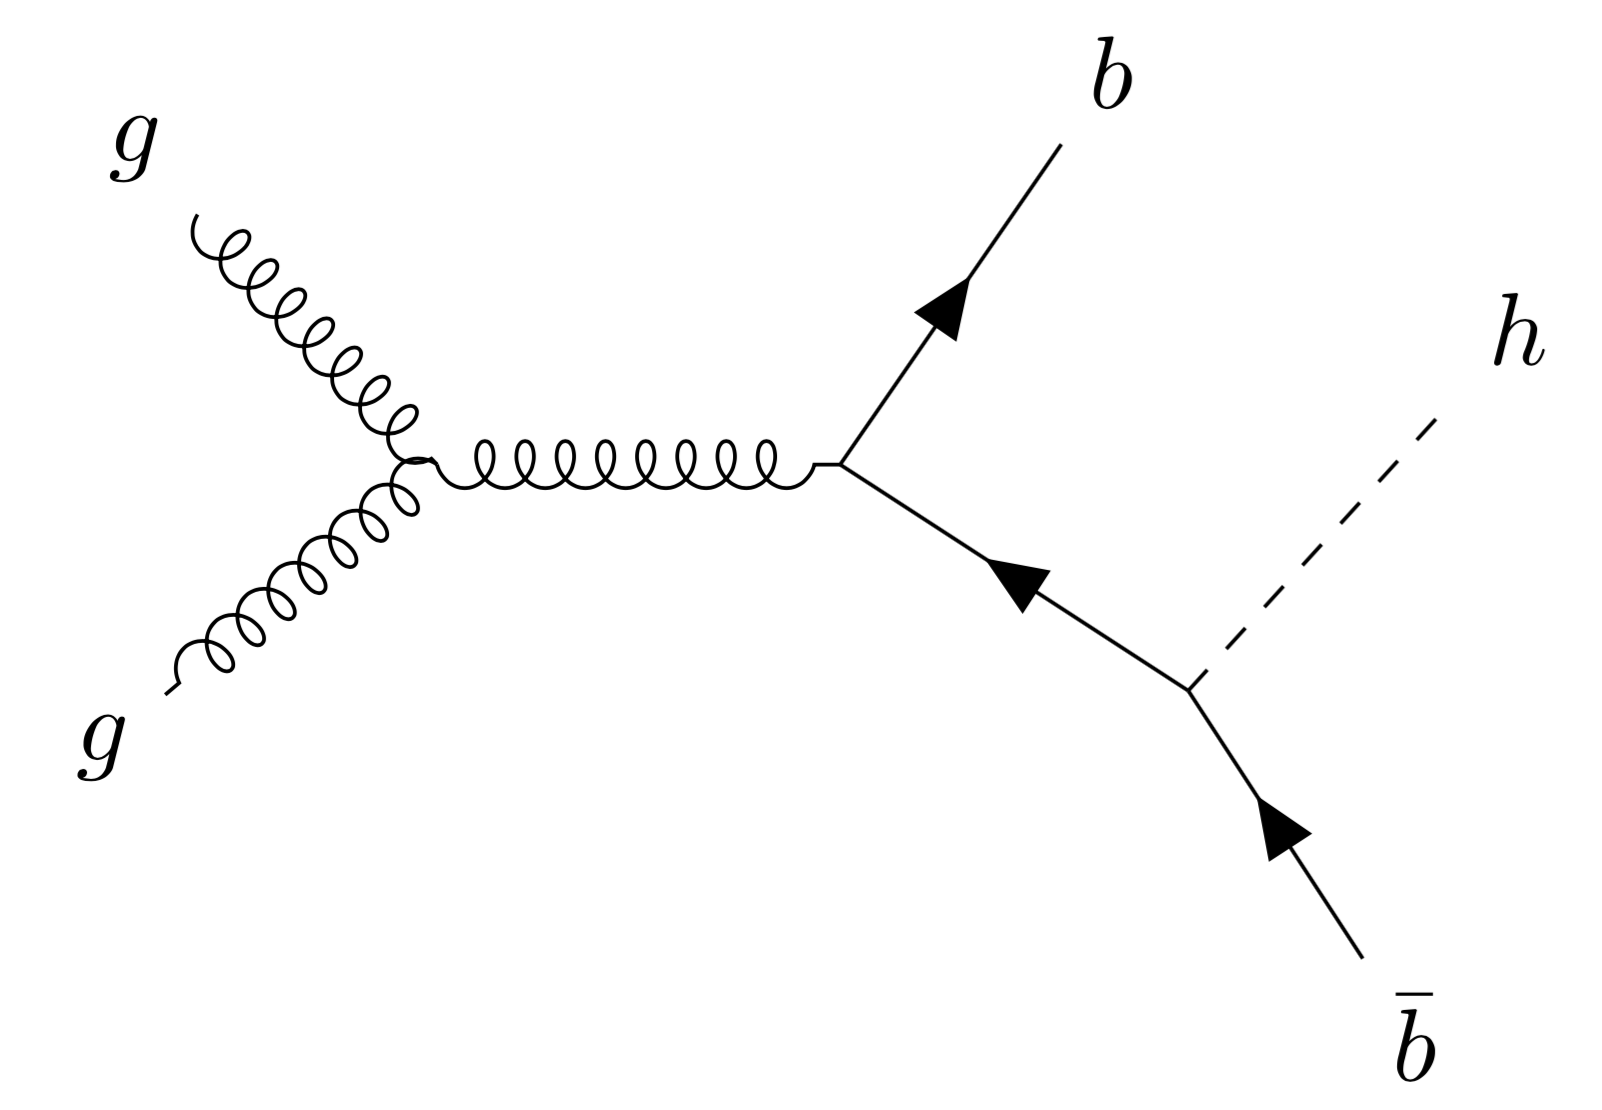
\includegraphics[height=10em]{bbhRad}\label{bbH1}}\hspace{2em}
  \subfloat[]{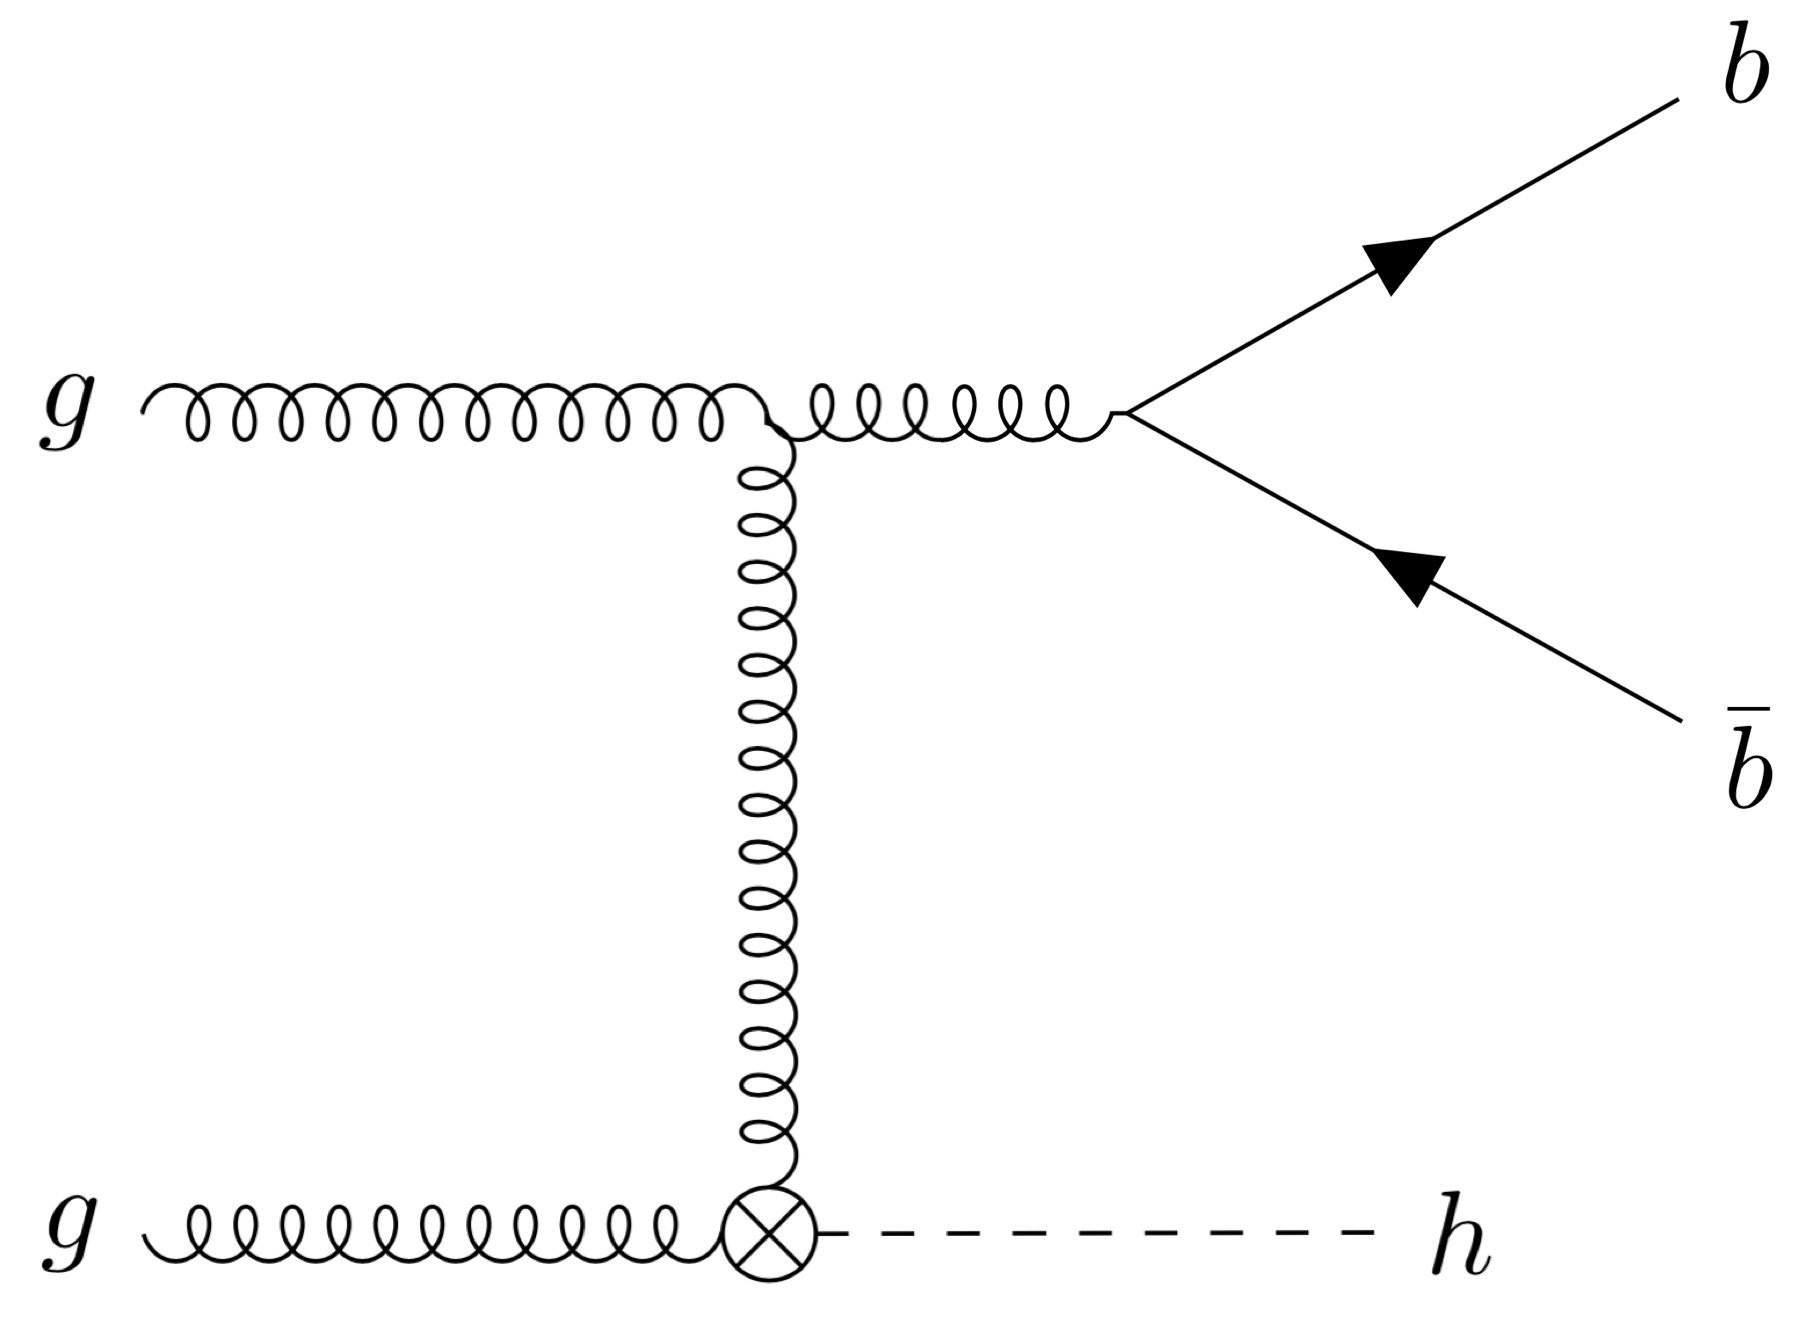
\includegraphics[height=10em]{bbhGF}\label{bbH2}}
  \caption[$pp\to H \bbbar$]{The two ways a Higgs boson can be produced in association to bottom quarks in the HEFT.}
  \label{bbHdiags}
\end{figure}

It is straightforward to see that the one-loop correction to Fig. \ref{bbH2} will scale like $\calo{y_t g_s^4}$, but we need to remember that the effect of integrating out the top quark to obtain the HEFT is not only to generate new interactions, but also to modify the SM interactions by power-suppressed corrections. In particular, the bottom Yukawa will receive a $1/m_t$ correction that scales like $\calo{g_s^4 y_t }$, meaning that the diagram in Fig. \ref{bbH1} is a piece of the calculation we are interested in. As a result, it is crucial to obtain this power-suppressed correction to the bottom Yukawa in the HEFT and this chapter we detail how it has been derived.

The easiest process we can use to extract this correction is the decay $H\to \bbbar$. In order to obtain a SM Feynman diagram for this process that has power-suppressed terms, we need to go to the two-loop level, as shown in Fig. \ref{hbb2l}. We need to compute the $1/mt$ expansion of these diagrams and match them to the relvant HEFT diagrams in order to extract the desired correction to the bottom Yukawa.

\begin{figure}[!h]
  \centering
  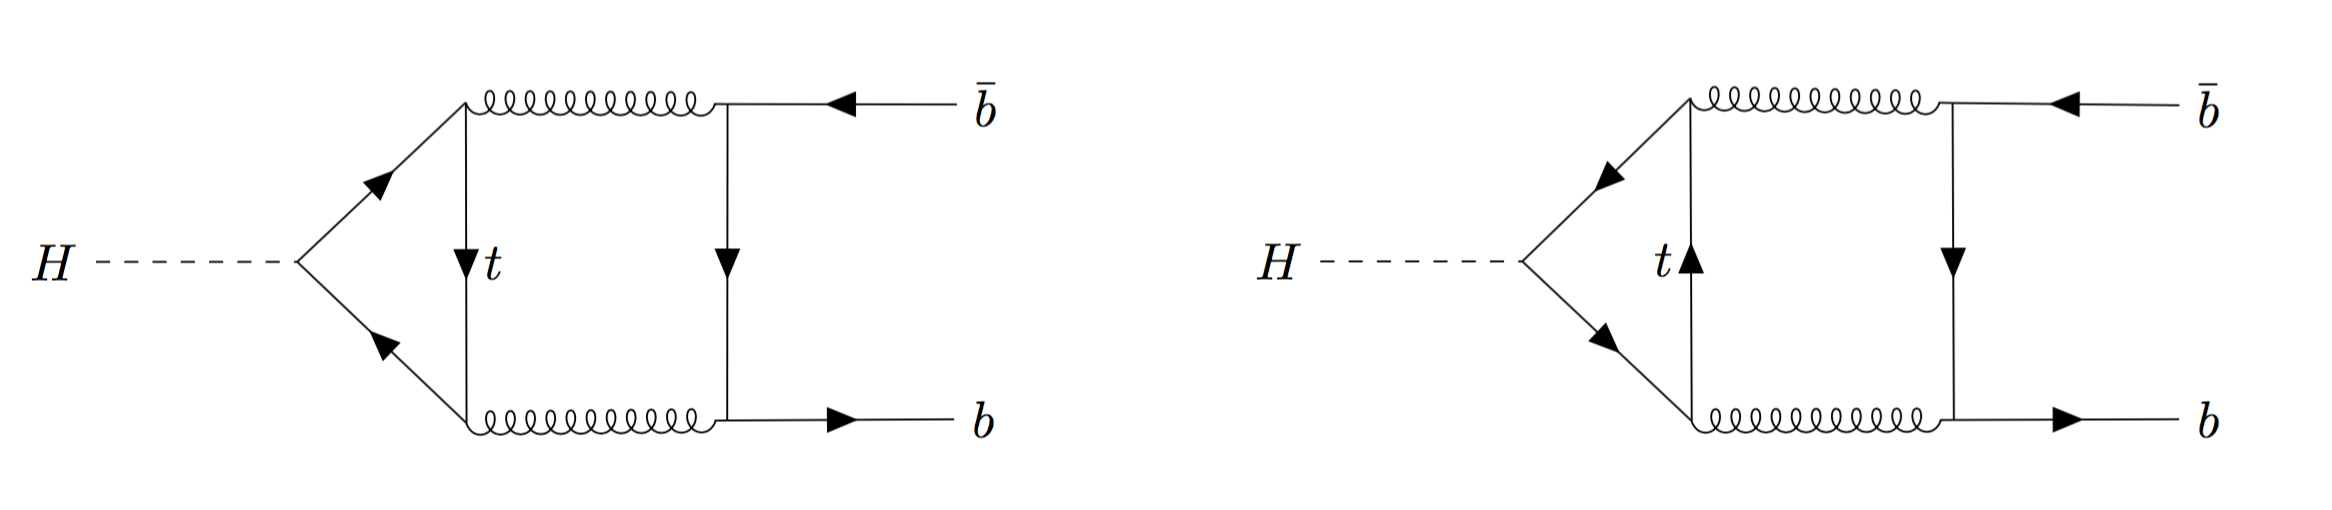
\includegraphics[width=\textwidth]{hbb2l}
  \caption[$H\to \bbbar$ at two loops in the SM]{The two $\calo{y_t g_s^4}$ diagrams that contribute to $H\to \bbbar$}
  \label{hbb2l}
\end{figure}

In the first section, we will perform the easier HEFT calculation, which involves both a tree-level and a one-loop diagram. Section 2 will then be dedicated to the calculation of the corresponding two-loop process in the SM in a $1/mt$ expansion and Section 3 will consist of comparing the two results to extract the finite and divergent parts of the required Wilson coefficient.
